\documentclass{whutmod}
\usepackage{metalogo}
\usepackage{float}
\usepackage{subfigure} 
\usepackage{url}
\usepackage[style=caspervector,backend=biber,utf8]{biblatex}
\addbibresource{wenxian.bib}
\team{38B}	% 组号
\membera{刘子川}
\joba{编程}
\memberb{程宇}
\jobb{建模}
\memberc{侯绍博}
\jobc{建模}
\hypersetup{
	colorlinks=true,
	linkcolor=black
}

\title{基于生命游戏算法对无人机探测路径进行优化}
\tihao{2} % 题号

\begin{document}
	
	\maketitle
	
	\begin{abstract}
   本文在网格分析的基础上使用“生命游戏”算法对无人机的探测巡查方案问题进行优化。对于两小时不间断的巡查问题,使用该模型分析存在可能的四种探测方案,并寻出最优解。最后用蜂巢密排模型来考虑巡查完成后的$1800m$以下区域的全覆盖问题。
   ~\\
   
   针对问题一,为对六架飞机飞行路线做出合理规划,采用分化网格的方式进行分析,再使用“生命游戏”算法对每架无人机的栅格数进行划分,并利用二分法精确划分区域。最后得出最短时间$t=5.89h$,覆盖率为94.97\%,并用仿真图对结果的合理性进行说明。
   ~\\
   
   针对问题二,为对该区域进行连续24h全面覆盖侦查,采用第一问的算法类比从而进行优化调度。分别计算出每次派遣五、六、七、八架无人机时所需的时间为$6.98h$、$5.89h$、$4.97h$、$4.37h$,连续24小时巡查需要派出的班次总数分别为4、4、3、3次。得出每次派遣五架无人机时,覆盖侦查需要最少无人机数量为$20$架,并给出每架无人机的探测巡查方案。
   ~\\
   
   针对问题三,为保证$1800m$以下区域进行信号全覆盖,将网格转换为蜂巢密排模型。先将蜂巢的每一个室的中点视为无人机,排满整个信号覆盖空间;其次设计无人机的循环运动路线,保证在运动过程中使信号正常覆盖,最后对覆盖精度进行了检测。
   ~\\
   
   本文的优点有两点:一是用生命游戏算法逼近真实解,还原出整个无人机飞行路径,且结果具有较高的准确性;二是利用优化网格划分,将蜂巢面代替覆盖面积,保证了运动过程中覆盖区域的密排性和连续性。
  
		\keywords{网格分划\quad  生命游戏算法\quad  最小二分法\quad  蜂巢密排模型}
		
	\end{abstract}
	
	%目录
	\tableofcontents
	\newpage	%换页符
	
	\section{问题重述}
	\subsection{问题的背景}

	无人机(UAV),是利用无线电遥控器和自备的程序控制装置操纵的不载人飞机,或者由车载计算机完全地或间歇地自主地操作。无人机在军用、民用等方面有着广泛的应用,并且在各行各业发挥着重要的作用。
	
	无人机与传统人力信息传递相比,有以下较为突出的特点 :能够避免飞
	行员在危险环境下作业,具有伤亡率低甚至零伤亡的特点;无需考虑机载生命的
	影响,为进一步实现飞行器的机动性、低可探测性、持续作战能力等提供了可能;
	降低了飞行器系统的复杂性,使其研发、制造、装备、使用和维护的难度和成本
	大大低于有人机;激发和拓展更多样的任务形式和使用需求等\parencite{pasko2016unmanned}。
	
	对于无人机来说,无人机航路规划的目标是在适当时间内计算、选择最佳的飞行航路。无人机的侦查问题本质上就是规划航路的问题,它既要保证侦查的覆盖率尽可能要大,又要合理利用侦查资源,节约成本。

	
	\subsection{问题概述}
	
	围绕无人机探测优化,依次提出如下问题:
	
	\begin{itemize}
		\item [(1)]
		 六架无人机对目标进行探测,给出起落时间、飞行路线,要求时间最短、覆盖率高的双目标优化问题;
		\item [(2)] 
		对该地区进行$24$小时不间断的全面侦查,且两次巡查的间隔不超过两小时,求最少的无人机数量
		\item [(3)] 海拔$3000m$高度的无人机可以保障$5000m$以内的设备通信,无人机之间的通信距离为$8000m$,要求$1800m$以下的区域全覆盖,求每架无人机的飞行路线。
	\end{itemize}
	
	\section{模型的假设}
	\begin{itemize}
		\item 无人机可以垂直起飞垂直降落;
		\item 无人机相互之间不会发生碰撞;
		\item 无人机可以一直保持最大速度飞行;
		\item 无人机移动步数时存在于划分网格的正中央。
	\end{itemize}
	
	
	\section{符号说明}
	\begin{center}
		\begin{tabular}{cc}
			\hline
			\makebox[0.3\textwidth][c]{符号}	&  \makebox[0.4\textwidth][c]{意义} \\ \hline
			$S$	    &  探测角覆盖面积 \\ \hline
			$r$	    &  覆盖面积半径 \\ \hline
			$s$	    &  转弯时划过面积 \\ \hline
			$R$  &  无人机转弯半径\\ \hline
		$\alpha $   &  无人机转弯角\\ \hline
			$d$	    & 无人机初始生命值  \\ \hline
		    $l_{n}$	& 分块网格间走的路程 \\ \hline
		    $\Delta H$	& 相邻网格高度差 \\ \hline
		    $\beta $ & 爬升/俯冲角\\ \hline
		\end{tabular}
	\end{center}
		%\subsubsection{模型建立与求解}
	\section{预备工作}
	\subsection{单架无人机的最优高度分析}
	
	由题目中所给定的无人机探测距离和最大视角得到分图,如下图~\ref{img}~所示:
	\begin{figure}[H]
		\centering
		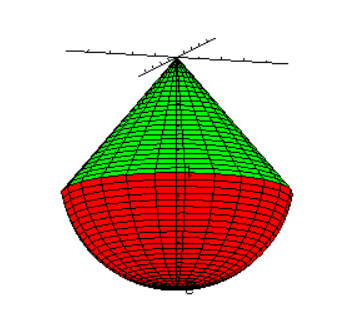
\includegraphics[width=.6\textwidth]{figures/1.png}
		\caption{无人机最大视角侧视图}\label{img}
	\end{figure}


	覆盖半径与无人机距离地面的函数关系式如下:
	\begin{gather}
	%	gather(代编号) 和gather*(不代编号) 环境(可使用\\换行)
		S(h) = \left\{\begin{matrix}
		\pi h^{2} & (0<h\leqslant 250\sqrt{2})\\ 
		\pi (r^{2}-h^{2})& (250\sqrt{2}<h\leqslant 500)\\ 
		0& (h>500)
		\end{matrix}\right.
	\end{gather}
	
	其中$S$为无人机探测角覆盖面积,$h$为无人机飞行高度。
	函数得出当飞行器距离地面$500*2^{\frac{1}{2}}\doteq 707m$时得到对于正下方区域的最大探测面积,此时探测半径$r$约为$353m$。
	
	\subsection{单架无人机的转向分析}
	当无人机转弯时可画出如下示意图:
	\begin{figure}[H]
		\centering
		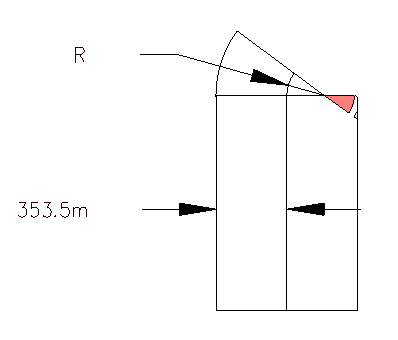
\includegraphics[width=.7\textwidth]{figures/zhuanwan.png}
		\caption{无人机转向分析图}\label{zhuanwan}
	\end{figure}
	
	其中,当转向半径大于覆盖$r\doteq 353m$时无人机移动时划过面积$s$表示如下:
	\begin{gather}
	s=\frac{\alpha (R+r)^{2}}{2}-\frac{\alpha (R-r)^{2}}{2}
	\end{gather}
	即:
	\begin{gather*}
	s=707\alpha R
	\end{gather*}
	其中$r$为覆盖半径,$R$为转弯半径,$\alpha $为转弯角,如图~\ref{ssss}~所示:
		\begin{figure}[H]
		\centering
		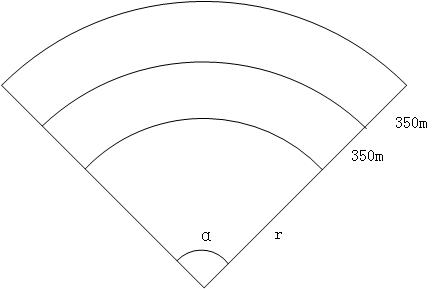
\includegraphics[width=.4\textwidth]{figures/sss.jpg}
		\caption{转角损失示意图}\label{ssss}
	\end{figure}
	
	
	此时走过的路径$l=\alpha r{}'$,面积与路径比$\lambda =\frac{s}{l}\doteq707$。当走直线时,面积$s=707x$,走过路径$l=x$。
	而当转向根据分析和计算可知半径小于r时,显然有面积损失;
	
	即应当尽量使转弯半径大于$353m$。
	
	\subsection{网格的划分}
	为了简化问题,将附件中给出的矩阵分块成以$14*14$小矩阵为元素的分块矩阵,
	然后将每个$14*14$的小矩阵上的点取平均值作为该位置的高度值;其中由于$2000m$为飞行最大高度,我们将海拔大于$2000m$的分块矩阵设值为$-1m$标记。
	得到简化后的等高图如图~\ref{img001}~所示:
	\begin{figure}[H]
		\centering
		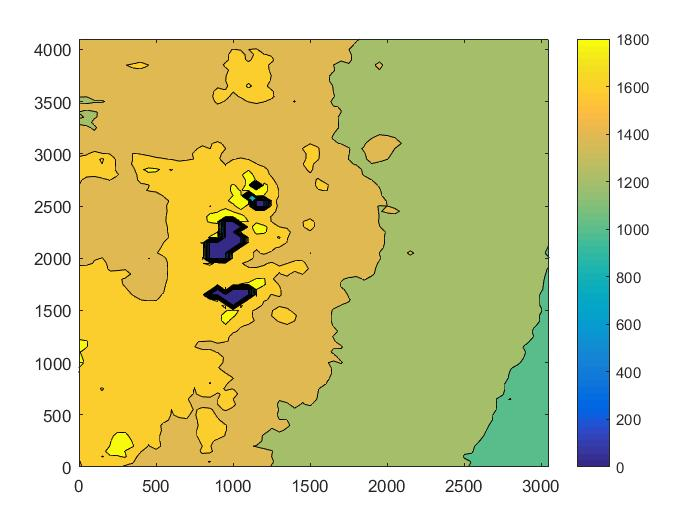
\includegraphics[width=.9\textwidth]{figures/2.jpg}
		\caption{分块划分后的等高图}\label{img001}
	\end{figure}
	
	\paragraph{在网格中的探测效率}
	由于将探测半径选取为2r,在网格中按照同一行或同一列飞行时,无人机有最大的探测效率,示意图如~\ref{zhuanxiang}~、~\ref{zhuanxiang1}~所示:
	
	\begin{figure}[H]
		\begin{minipage}[t]{0.5\linewidth}
			%并排插图时,线宽很重要,自己慢慢试,俩张图就不要超过0.5,三张图不要超过0.33之类的,自己看着办
		\centering
		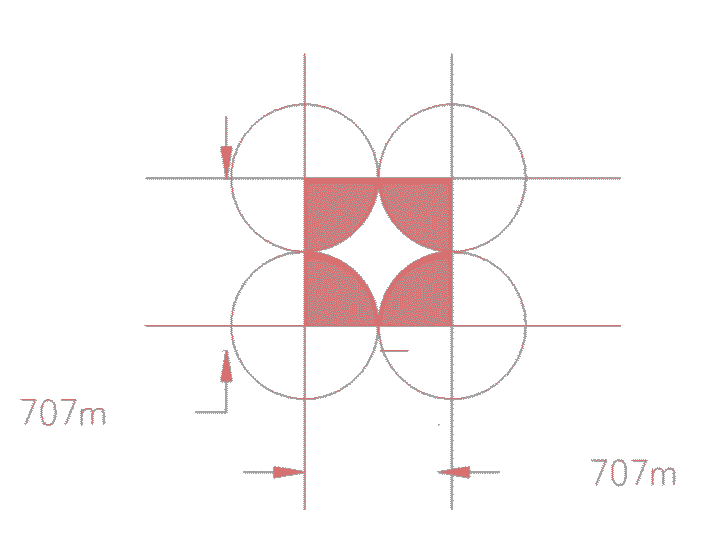
\includegraphics[width=\textwidth]{figures/zhuanxiang.png}
		\caption{面积利用率说明图}\label{zhuanxiang}
		\end{minipage}
		\hfill%分栏的意思吧
		\begin{minipage}[t]{0.5\linewidth}
		\centering
		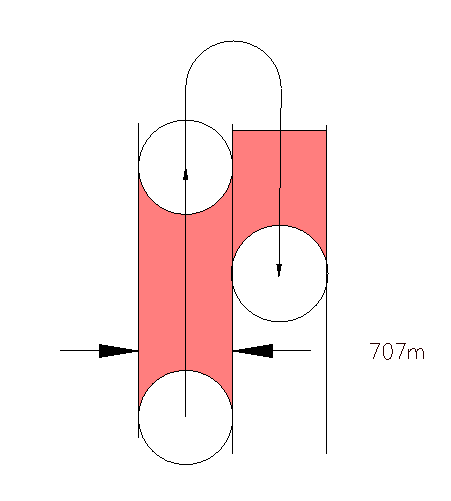
\includegraphics[width=\textwidth]{figures/zhuanxiang2.png}
		\caption{直线飞行示意图}\label{zhuanxiang1}
		\end{minipage}
	\end{figure}

	即当无人机移动过程中沿直线行走时,可使覆盖面积最大。
	
	\paragraph{在网格中的转向问题}
	在网格中进行90°转向时,可以令取转向半径为最短的转向半径从而可以使移动路程约等于在直角中转弯所移动的路程,如图~\ref{90zhuan}~所示。

	\begin{figure}[H]
		\centering
		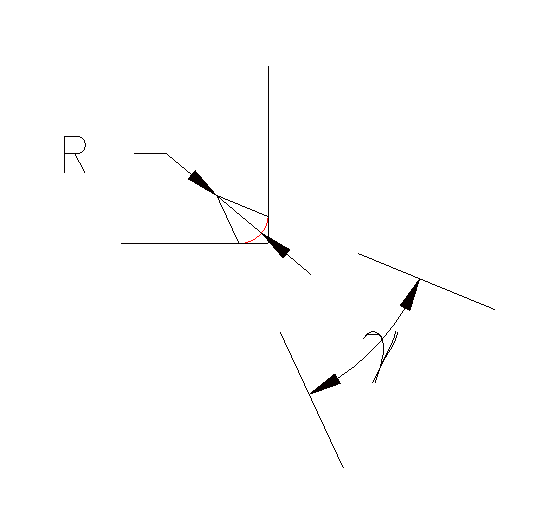
\includegraphics[width=.5\textwidth]{figures/90zhuan.png}
		\caption{无人机90°转向分析}\label{90zhuan}
	\end{figure}

	由图~\ref{90zhuan}~可知,网格中的直角转弯可以近似为弧角转弯,且经计算弧角转弯损耗距离略大于直角转弯,因此可用直角转弯代替实际无人机的弧角转弯,从而简化模型。

	
	\section{问题一模型的建立与求解}
	\subsection{问题一描述与分析}
	%\subsubsection{问题一描述与分析}
	针对问题一,要求用最短的时间完成对整个区域的探测任务,对6架无人机的飞行方案做出规划,在尽可能短的时间内对于尽可能大的覆盖面积进行探测,故需要建立一个优化模型求解。
	
	考虑到无人机的探测面积与无人机距离地表高度相关,为了简化问题,将目标区域划分成方格图,并依照附件二中的区域高程数据划画出简化等高线,再通过本组设计的“生命游戏”算法对完全探测使用的最小时间进行优化求解。

	\subsection{模型的建立与求解}
	多架无人机同时出发,由于该问题的最短时间反应了多架无人机的一种短板效应,即最后返回无人机的返回时间决定了整个探测所使用的总时间。
	
	\paragraph{算法描述}
	假设无人机按照恒定的最大速度飞行,因此不妨假定所有无人机依次出发,其生命游戏算法描述如下:
	
	\begin{itemize}
		\item [(1)]
		令每一架无人机所走过的路程都等于初始生命$d$,且经过的路径不与上一架无人机重合;
		\item [(2)] 
		无人机出发后每走一格网格消耗一定行动能力,从而减少生命值;
		\item [(3)] 当第n架无人机达到极限生命时记录位置并沿欧氏距离返航;
		\item [(4)] 第n+1架沿欧氏距离飞回,递归执行步骤(2),直到填满网格;
			\item [(5)] 当探测区域被完全覆盖时(且所有的无人机安全返航),若此时还有剩余无人机或最后一架无人机的返航后生命值$d>0$,则减小初始生命$d$的取值再次重复上述步骤;
			\item [(6)] 通过二分法得到一个符合精度要求的d的取值后,结束程序。
\end{itemize}
	
	模型可以用以下流程图表示如下:
	\begin{figure}[H]
		\centering
		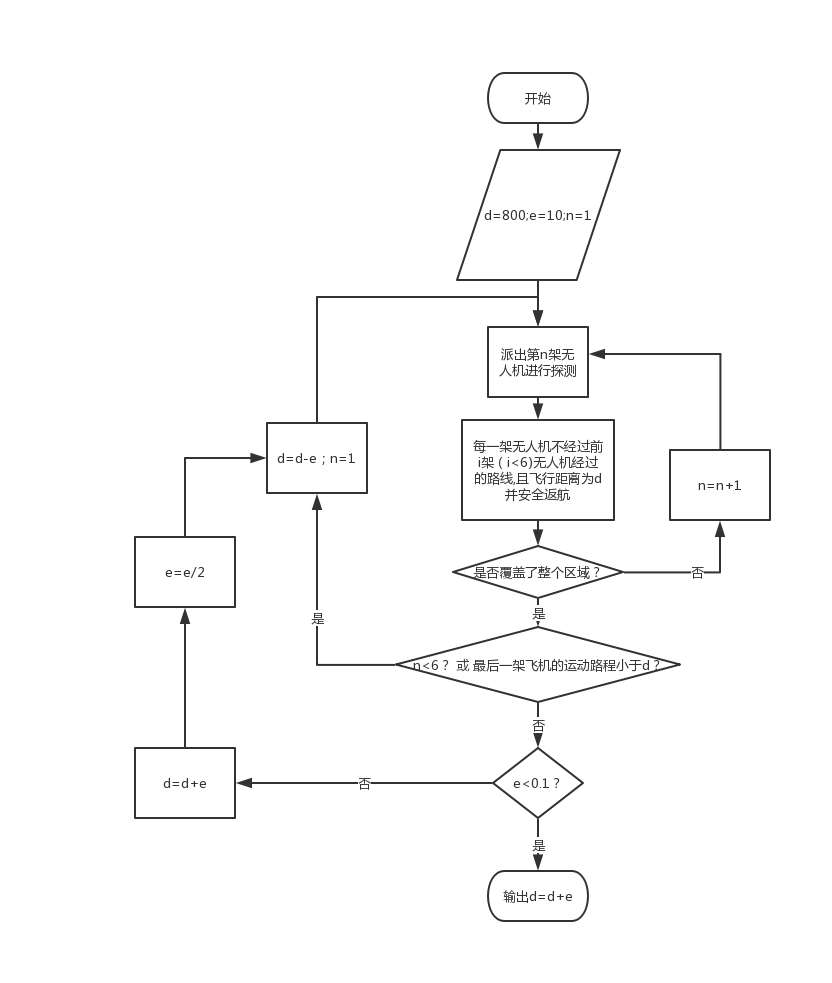
\includegraphics[width=\textwidth]{figures/lct.png}
		\caption{生命游戏算法流程图}\label{lct}
	\end{figure}

	为了确保无人机安全,首先去除所有矩阵中高程在2000m以上的数值点得到安全的飞行区域。将矩阵中的高程数据转化为飞行高度数据,并将区域划分成等面积的两半,分别从A和B分别派出无人机\parencite{田春颖2004基于栅格地图的移动机器人完全遍历算法},采用机器人完全遍历中的遍历移动方式,如图~\ref{qq}~所示:


	\begin{figure}[H]
		\centering
		\subfigure[pic1.]{
			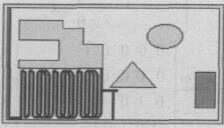
\includegraphics[width=5.5cm]{q.jpg}
			%\caption{fig1}
		}
		\quad
		\subfigure[pic2.]{
			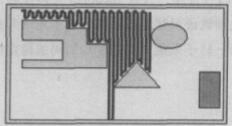
\includegraphics[width=5.5cm]{qq.jpg}
		}
		\quad
		\subfigure[pic3.]{
			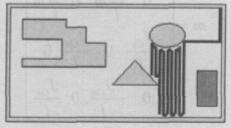
\includegraphics[width=5.5cm]{qqq.jpg}
		}
		\quad
		\subfigure[pic4.]{
			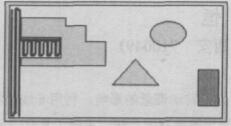
\includegraphics[width=5.5cm]{qqqq.jpg}
		}
		\caption{ pics}\label{qq}
	\end{figure}
	
	该算法中的每一架无人机都是依次出发且不与(或尽量的少与)已经返回的无人机所经过的路径相重合,由此算出所有无人机所飞行的路线。在实际操作中,使所有的无人机同时起飞,按照该算法所得出的路线同时起飞后进行探测任务,最终可以使每一架无人机飞过的路程尽可能的短,从而整个探测任务消耗的时间最短。

	根据算法描述,可设立以下优化函数与约束方程:
	\begin{gather}
		z=d \\
		st. \left\{\begin{matrix}
		\sqrt{[x(t)-x_{i}]^{2}+[y(t)-y_{i}]} \leqslant d-E& i=a,b\\
		E=\int_{t}^{0} \sqrt{x^{2}(t)+y^{2}(t)}dt\\ 
		X=x(t)& \\ 
		Y=y(t)& 
		\end{matrix}\right.
	\end{gather}
	
	其中,$X=x(t),Y=y(t)$是无人机行走的路线对应损失的生命,$d$为无人机初始生命值。
	
	
	
	\paragraph{高度差处理}当它从一个矩阵移动到另一个相邻矩阵时计算行动路程如图~\ref{gaodu}~所示:
		\begin{figure}[H]
		\centering
		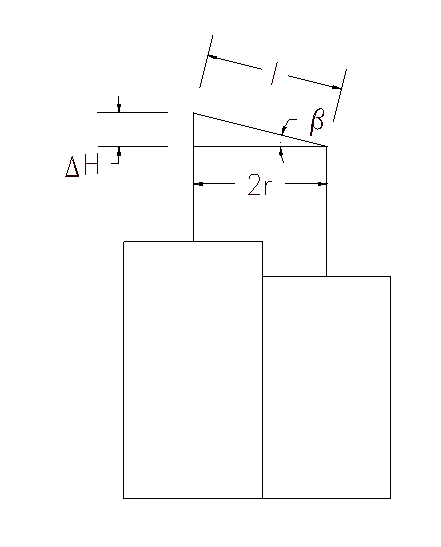
\includegraphics[width=.5\textwidth]{figures/gaodu.png}
		\caption{相邻矩阵行动路程示意图}\label{gaodu}
	\end{figure}


	考虑到无人机的爬山角度和俯冲角度不得大于15°,当相邻矩阵间$\frac{H_{i}-H_{j}}{2r}>tan15^{\circ}$时,可令$D=\infty$表示此路通不过。

	即可计算出相邻矩阵行动损失的生命为:
	\begin{gather*}
		l_{n}=\sqrt{(2r)^{2}+\Delta H^{2}}
	\end{gather*}

	其中$l_{n}$为网格间走的路程,$\Delta H=\left | H_{i}-H_{i+1} \right |$为网格间高度差,从而已经走过的总路程可求和表示为:
	
	\begin{gather}
	L_{n}=\sum_{n=1}^{N}l_{n}
	\end{gather}

		\paragraph{二分法确定生命周期}人工设定参数e,当$L_{n}<d$时生命消耗完,无人机返航并沿原路派出下一架无人机,接替上一架无人机沿设定轨迹继续按照设定路线进行探测行动,当探测完成后若最后一架无人机行动距离满足$L_{n}<d$时,则有减小$d$,使$d=d-e$,重复上述步骤。直到无人机不能遍历整个探测区域时,减小$e$,使得$e=\frac{e}{2}$,重复上述直到当$e<0.1$时停止算法输出所需最小生命$d$。
	
	\paragraph{计算覆盖率}
	考虑到无人机最大视角和离地高度之间存在限制问题,即当无人机大于约$1650m$后,无法达到最大视角,即可分类讨论海拔与覆盖面积的关系,如图~\ref{fugailv}~所示:
	
		\begin{figure}[H]
		\centering
		\subfigure[小于1650m]{
			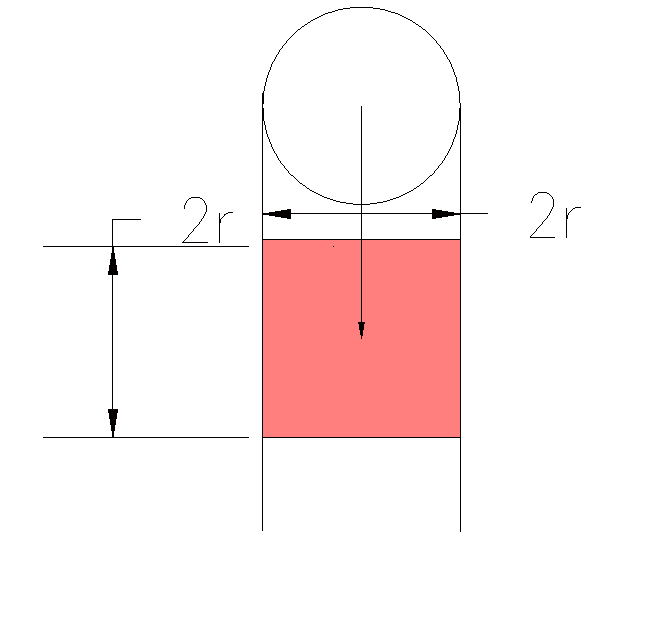
\includegraphics[width=6.5cm]{figures/yy.png}
			%\caption{fig1}
		}
		\quad
		\subfigure[大于1650m]{
			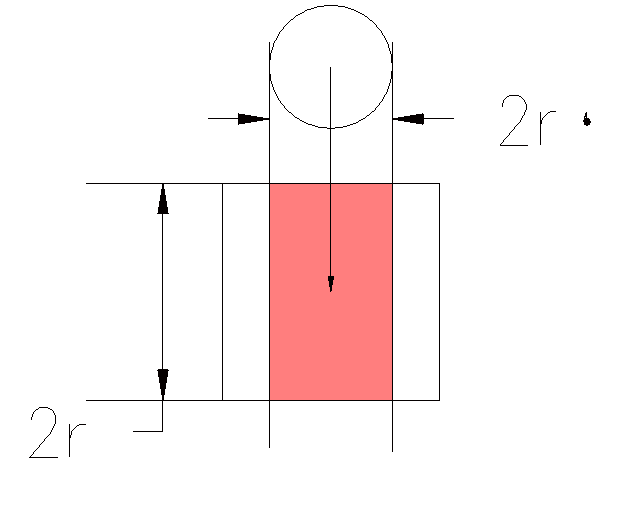
\includegraphics[width=6.5cm]{figures/yyy.png}
		}
		\caption{海拔与覆盖面关系图}\label{fugailv}
	\end{figure}
	
	可得到每个矩形格中的覆盖率的面积与海拔的关系式为:
	\begin{gather}
	S=\left\{\begin{matrix}
	500000& H\leqslant 2000-250\sqrt{2}\\ 
	500\sqrt{2}*(4000-2H) & 2000-250\sqrt{2}<H<2000
	\end{matrix}\right.
	\end{gather}
	
	则总的覆盖面积为:$\sum_{n=1}^{N}S=2415.31km^{2}$,其覆盖率为:94.966\%
	
	
	
	\paragraph{探测结果}得出优化路径仿真结果如图~\ref{imgxxxx}~~\ref{imgxxxxx}~所示:
	
	\begin{figure} [H]
		\centering 
		\subfigure[pic1.]{% 
			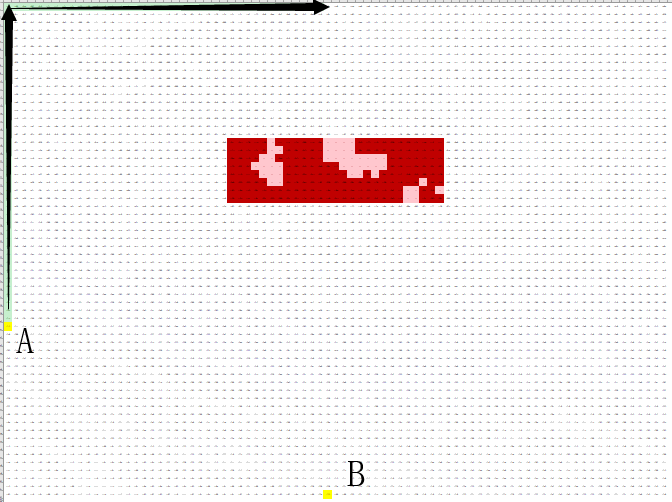
\includegraphics[width=5cm]{figures/11.png}}
		\quad
		\subfigure[pic2.]{% 
			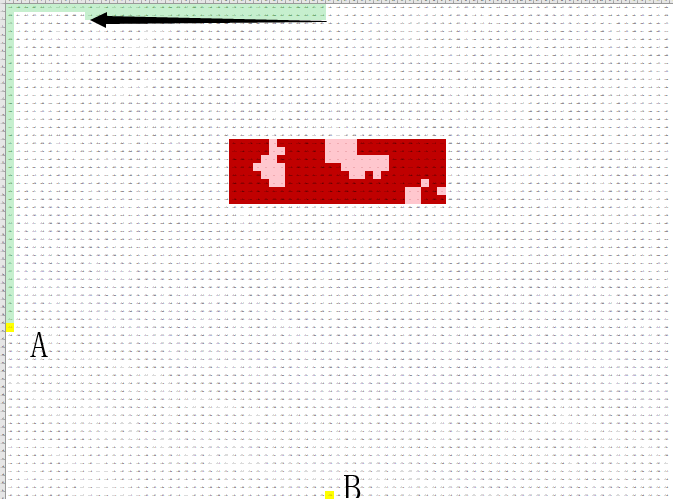
\includegraphics[width=5cm]{figures/22.png}}
				\quad
		\subfigure[pic3.]{
			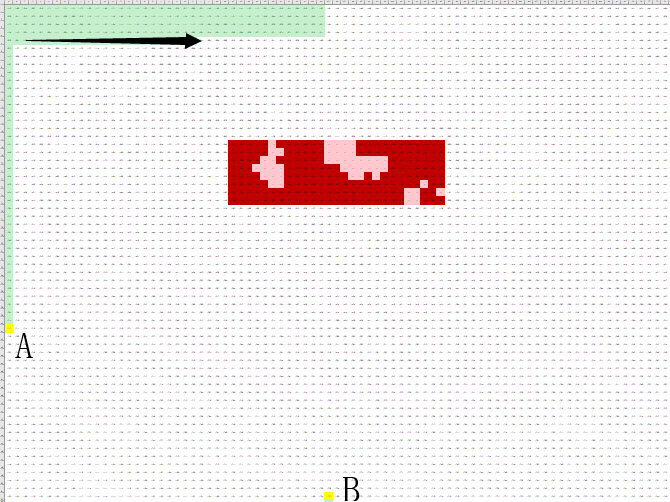
\includegraphics[width=5cm]{figures/33.png}
		}
		\quad
		\subfigure[pic4.]{
			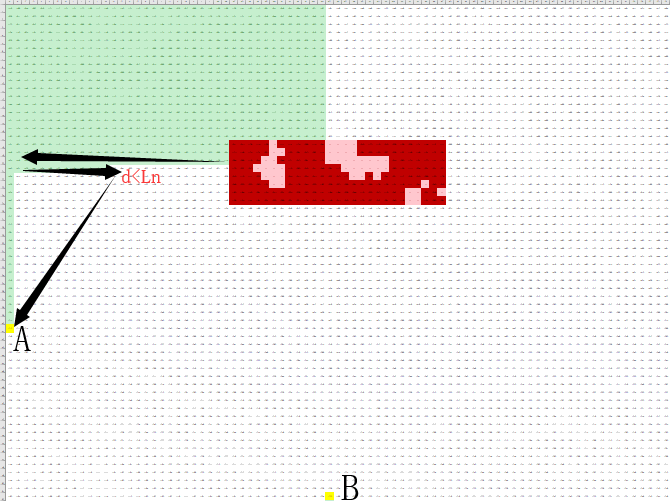
\includegraphics[width=5cm]{figures/44.png}
		}
	\end{figure}

	\addtocounter{figure}{-1}       %先欺骗LaTeX图形计数器
	\begin{figure} [H]
		\addtocounter{figure}{1}      %再告诉LaTeX图形计数器真相
		\centering 

		\quad
		\subfigure[pic5.]{
			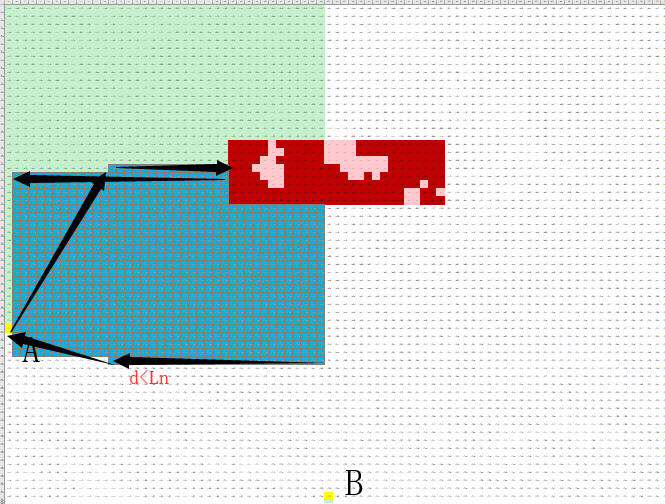
\includegraphics[width=5cm]{figures/55.png}
		}
		\quad
		\subfigure[pic6.]{
			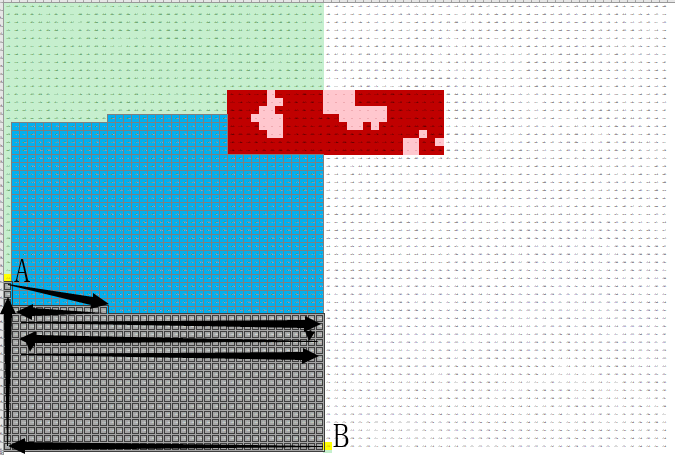
\includegraphics[width=5cm]{figures/66.png}
		}
		\caption{A块区域路径仿真结果图}\label{imgxxxx}
	\end{figure}

%	\begin{figure}[H]
%		\centering
%		\subfigure[pic1.]{
%			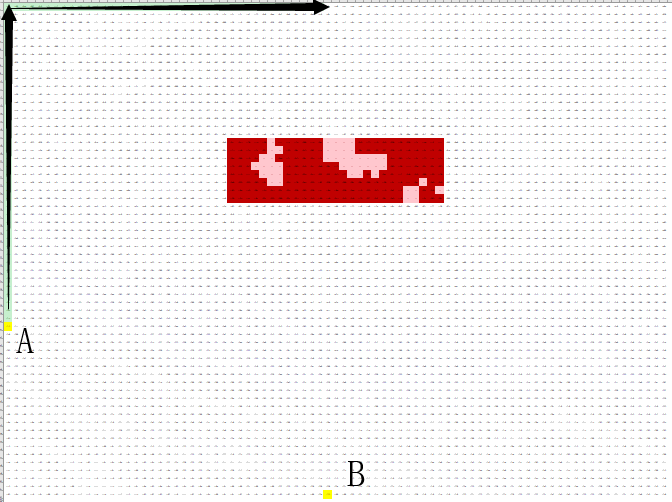
\includegraphics[width=6.5cm]{figures/11.png}
%			%\caption{fig1}
%		}
%		\quad
%		\subfigure[pic2.]{
%			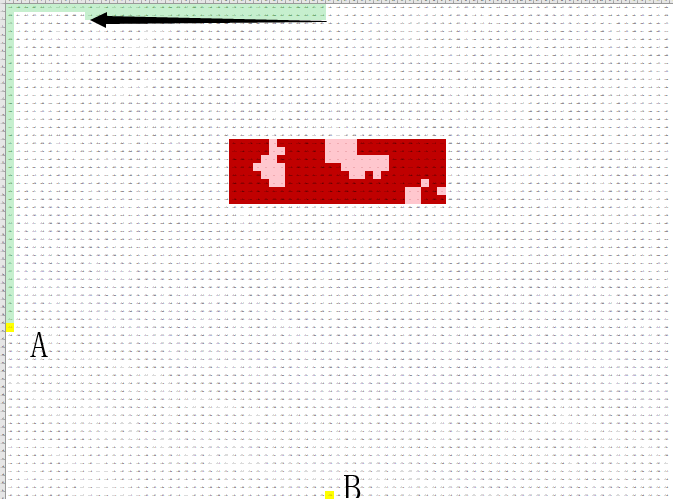
\includegraphics[width=6.5cm]{figures/22.png}
%		}
%		\quad
%		\subfigure[pic3.]{
%			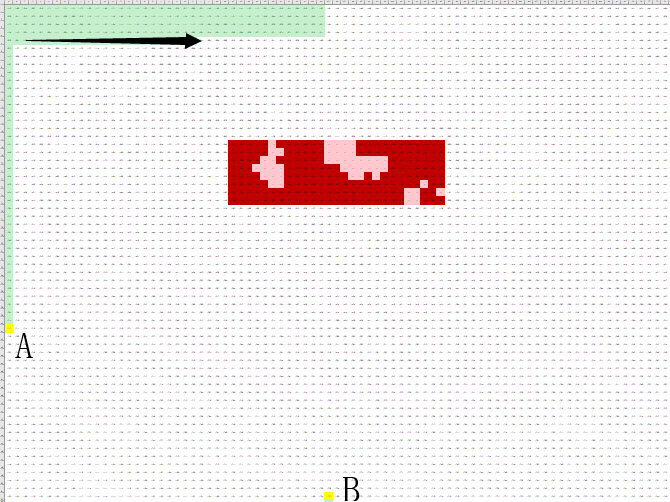
\includegraphics[width=6.5cm]{figures/33.png}
%		}
%		\quad
%		\subfigure[pic4.]{
%			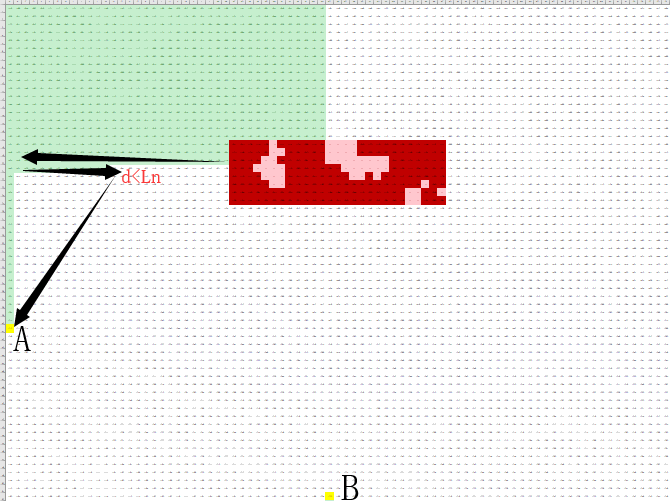
\includegraphics[width=6.5cm]{figures/44.png}
%		}
%		\quad
%		\subfigure[pic5.]{
%			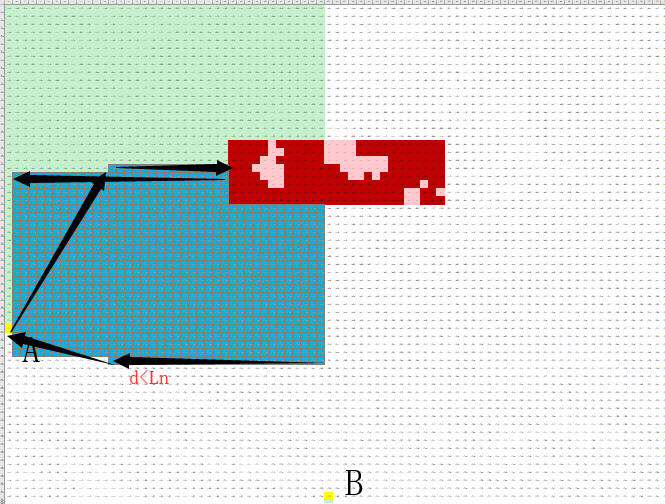
\includegraphics[width=6.5cm]{figures/55.png}
%		}
%		\quad
%		\subfigure[pic6.]{
%			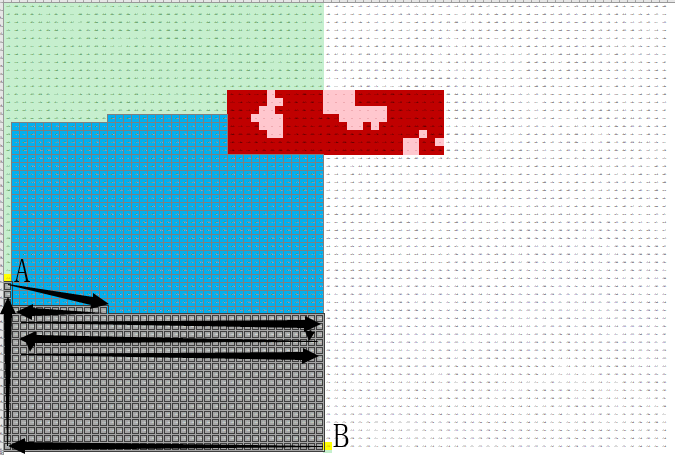
\includegraphics[width=6.5cm]{figures/66.png}
%		}
%		\caption{A块区域路径仿真结果图}\label{imgxxxx}
%	\end{figure}

	\begin{figure}[H]
		\centering
		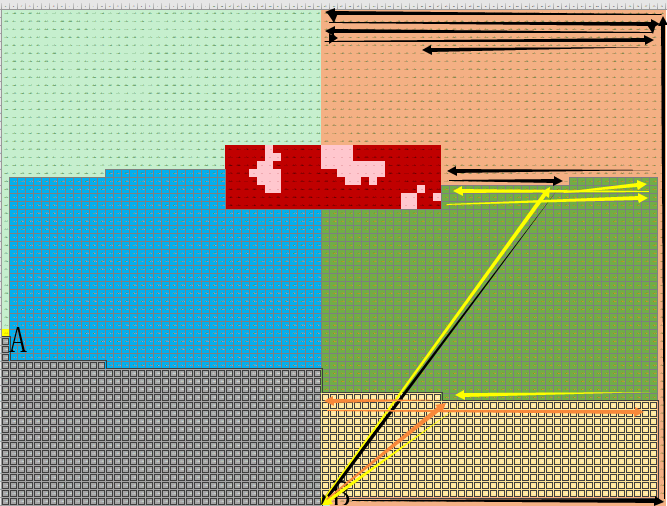
\includegraphics[width=.7\textwidth]{figures/77.png}
		\caption{B块区域路径仿真结果}\label{imgxxxxx}
	\end{figure}
	
	其覆盖率与所用时间见表~\ref{tab111}~:
	\begin{table}[H]
		\caption{覆盖率与所需时间}\label{tab111} \centering
		\begin{tabular}{ccccc}
			\toprule[1.5pt]
			覆盖面积 & 覆盖率 & 所需时间 \\
			\midrule[1pt]
		2415.31$km^{2}$	& 94.966\% &5.89795h\\
			\bottomrule[1.5pt]
		\end{tabular}
	\end{table}
	
	\section{问题二模型的建立与求解}
	\subsection{问题二描述和分析}
	需要使用最少数量的无人机,要求区域中的每个部分被,修改第一问模型,建立一个调度模优化型。

	修改问题一的模型依次计算$n(n=1,2,3,...)$架无人机探测目标区域所需要的最短时间,可以得到当每两个小时派出n架无人机所需要的总无人机数量$N(N<25)$,比较每个n对应的N的值,即可求得最小需要的无人机数量。

	\subsection{模型建立与求解}
	经估算得出当每两小时次派出5,6,7,8架飞机时总无人机总数N<25,即此时才能符合题目中的底线要求。
	修改问题一模型 ,计算出当n架无人机时(n=5,6,7,8)时,每次探测整个目标区域使用的时间为T。

	
	
	由此调整飞机个数得出调度规划图:
	\begin{figure}[H]
		\begin{minipage}[t]{0.5\linewidth}
		\centering
		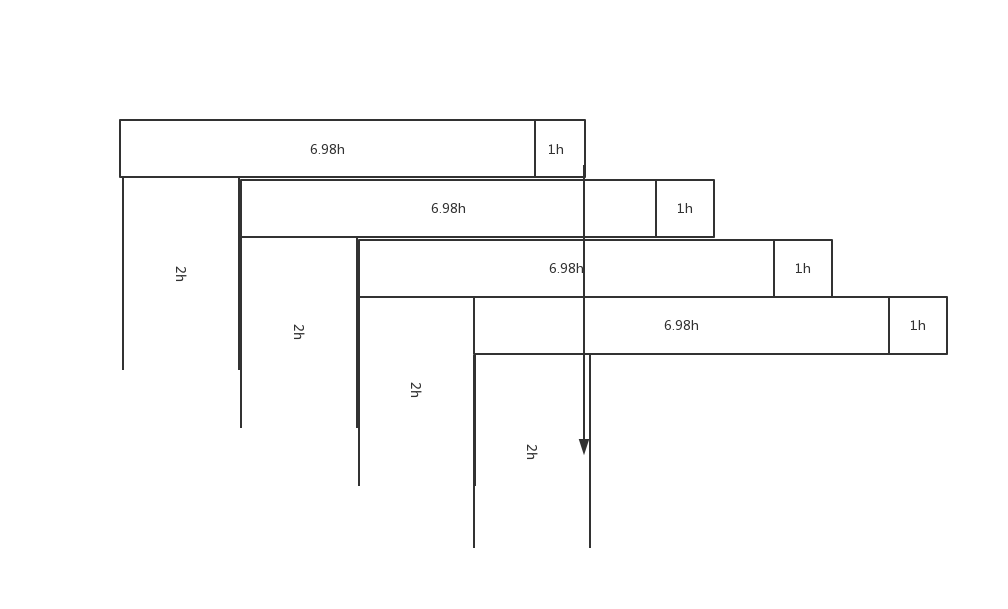
\includegraphics[width=\textwidth]{figures/5j.png}
		\caption{五架无人机调度规划图}\label{5j}
		\end{minipage}
		\hfill%分栏的意思吧
		\begin{minipage}[t]{0.5\linewidth}
		\centering
		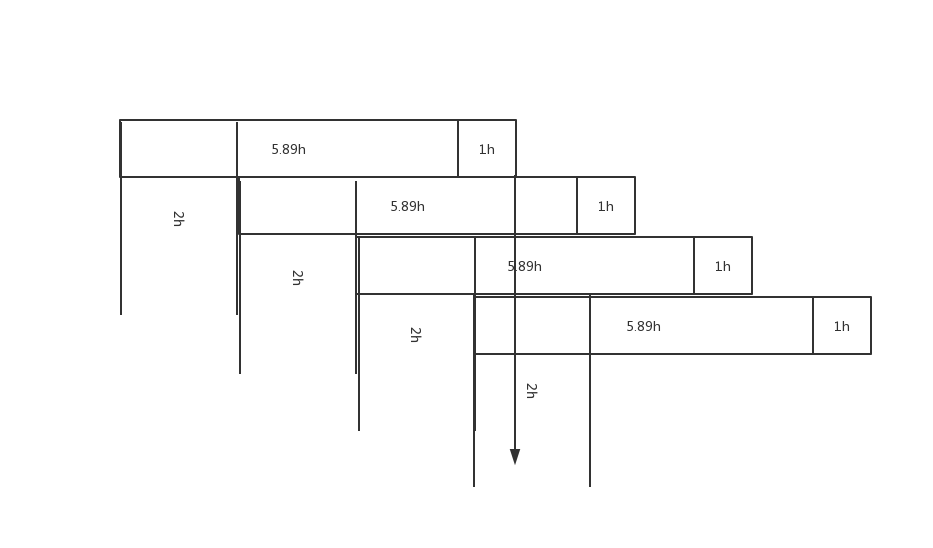
\includegraphics[width=\textwidth]{figures/6j.png}
		\caption{六架无人机调度规划图}\label{6j}
		\end{minipage}
	\end{figure}
	\begin{figure}[H]
	\begin{minipage}[t]{0.5\linewidth}
		\centering
		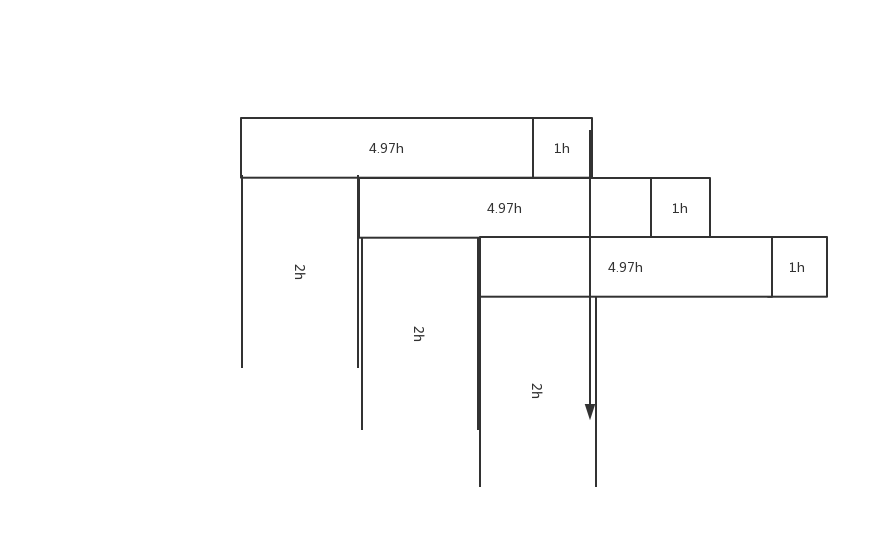
\includegraphics[width=\textwidth]{figures/7j.png}
		\caption{七架无人机调度规划图}\label{7j}
	\end{minipage}
	\hfill%分栏的意思吧
	\begin{minipage}[t]{0.5\linewidth}
		\centering
		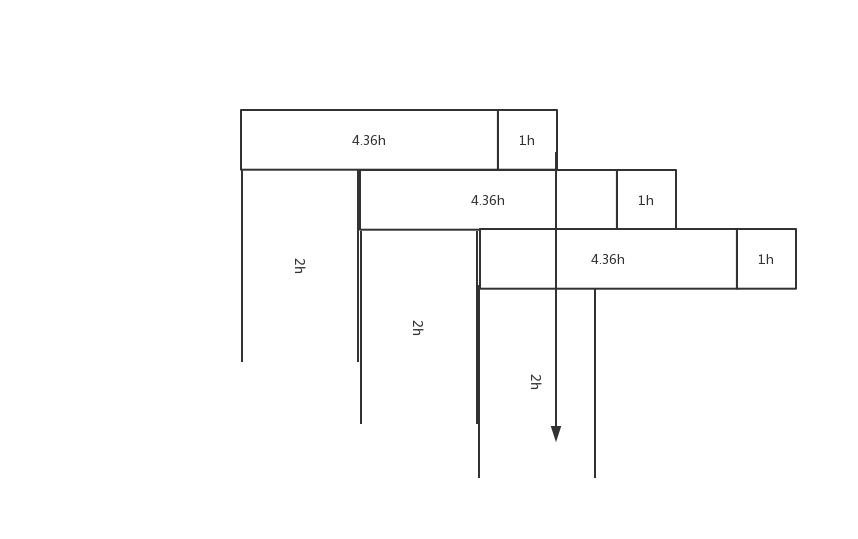
\includegraphics[width=\textwidth]{figures/8j.png}
		\caption{八架无人机调度规划图}\label{8j}
	\end{minipage}
\end{figure}
	如上图所示,当第一组无人机回到基地并可以再出发时;总共已经派出了$p$组无人机,即$p$组无人机就可以构成一个链式循环,总共使用无人机数$N=p*n$。根据算法描述,求得其调度结果与时间见表~\ref{labelll}~所示:
	\begin{table}[H]
	\caption{调度结果与时间}\label{labelll} \centering
	\begin{tabular}{ccccc}
		\toprule[1.5pt]
		单次派出个数 &派出组数&  所需共个数 & 所需时间 \\
		\midrule[1pt]
		五架	& 4 &20 &6.98246h\\
		六架	& 4 & 24 &5.89795h\\
		七架	& 3 &21 &4.9725h\\
		八架	& 3 &24 &4.36842h\\
		\bottomrule[1.5pt]
	\end{tabular}
\end{table}

	结果表明,其所需时间都小于$8h$,则当每两小时派遣五架无人机时,所需最少无人机数量为二十架。总的覆盖面积为:$2415.31km^{2}$,其覆盖率为:94.966\%,其各自的飞行探测巡查方案仿真图如下:
	
		\begin{figure}[H]
		\centering
		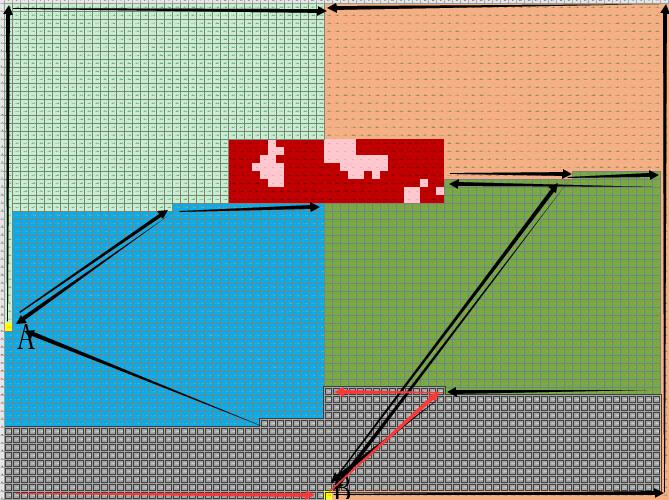
\includegraphics[width=.7\textwidth]{figures/88.png}
		\caption{各自的飞行探测巡查方案仿真图}
	\end{figure}
	
	\section{问题三模型的建立与求解}
	
	
	\subsection{问题描述和分析}
	  针对问题三,要求使用最少无人机数量使信号覆盖$1800m$以下的目标区域。改进网格形状的划分,为了简化问题,我们分别分析了三角形密排,正方形密排,正六边形密排。通过比较这三者的面积覆盖率得到一个面积密排优化模型。
	
	\subsection{模型的建立与求解}
	
	\paragraph{覆盖近似}
	由于要求所有区域连续不断地被覆盖,我们设计一个合理的飞机之间的距离,使得第一架飞机的信号刚好离开该区域时,后面一架飞机恰好覆盖到该区。
	
	单个无人机的覆盖范围是以无人机为圆心,$5000m$为半径的圆,但为了与周围的无人机组成紧密贴合的网,则只能以直线为边界,此时有效覆盖面积为圆内接最大正3、4、6边形,以直线运动为例,分别分析上述两架飞机到达的距离间隔,如图~\ref{llll}~所示。
	
	\begin{figure}[H]
		\centering
		\subfigure[pic1.]{
			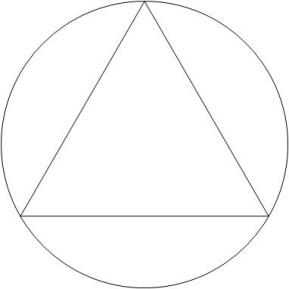
\includegraphics[width=4cm]{l.png}
			%\caption{fig1}
		}
		\quad
		\subfigure[pic2.]{
			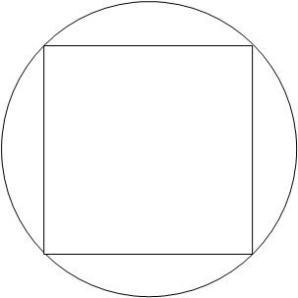
\includegraphics[width=4cm]{ll.png}
		}
		\quad
		\subfigure[pic3.]{
			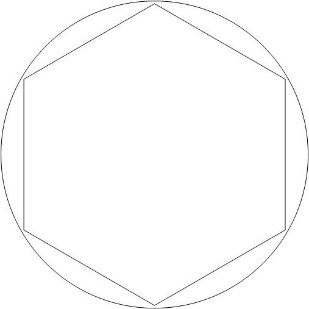
\includegraphics[width=4cm]{lll.png}
		}
		\caption{覆盖近似图}\label{llll}
	\end{figure}
	
	设覆盖半径$r=5000m$,图1可得正三角形中心距离边的距离为$\frac{1}{2}r$,此时相邻两飞机的间距为r.同理图2的相邻半径为$\sqrt{2}r$,图3相邻半径为$\sqrt{3}r$。
	
	
	由图~\ref{llll}~的圆内接六边形进行覆盖,具有近圆面积高83\%,保证飞机间距长等优点,明显能提高飞机利用率,减少飞机数量。
	\paragraph{无人机之间距离修正}
	计算得到的最近的两架无人机之间的距离为$8500m$,大于所给定的$8000m$,所以我们不妨取两架飞机的间距为$8000m$,再对覆盖半径进行等比例缩小。
	
	 模型建立可以分为两个步骤:第一,假设无人机是悬停状态,用最少的无人机实现无缝的覆盖;第二,给予悬停的无人机路线规划,使无人机进行循环运动。
		
	\paragraph{静态无缝覆盖}
	 假设无人机是悬停状态,用最少的无人机实现无缝的覆盖。则根据相对运动原理:无人机对区域的运动可以变成区域相对无人机的运动。
	 
	采取在边长为$4618.94m$正六边形无限大网格中,移动一个边长为$43.7*58.2$的带有去除$1800m$以上区域的长方形框(模拟在1800m以下区域中搜索无人机最小架数的过程),找出框中包含六边形中点最少的时刻,正六边形中点数及代表无人机的架数。
		
			\begin{figure}[H]
		\centering
		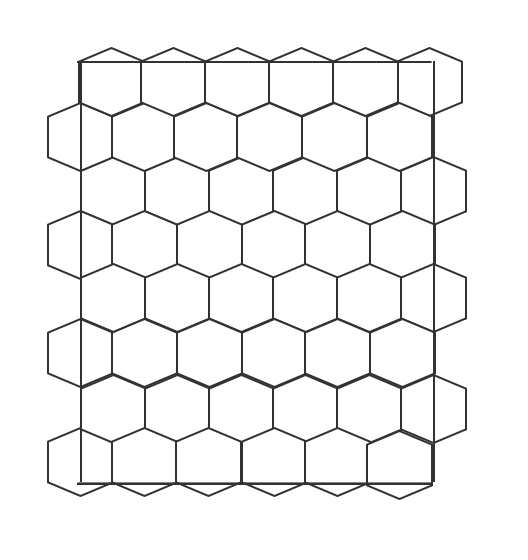
\includegraphics[width=.5\textwidth]{figures/jj.png}
		\caption{蜂巢无缝覆盖示意图}
	\end{figure}

\paragraph{循环运动}
让静态图中的六边形(无人机)动起来,为了简化分析,将每一横排设计成直线运动,当无人机运动到边缘时,转而移动到下一排。为了保证转弯处能被覆盖到,我们采取两排组网、覆盖面积有余量的边界处转弯的原则,进行环状运动,如图所~\ref{jjj}~示。
			\begin{figure}[H]
	\centering
	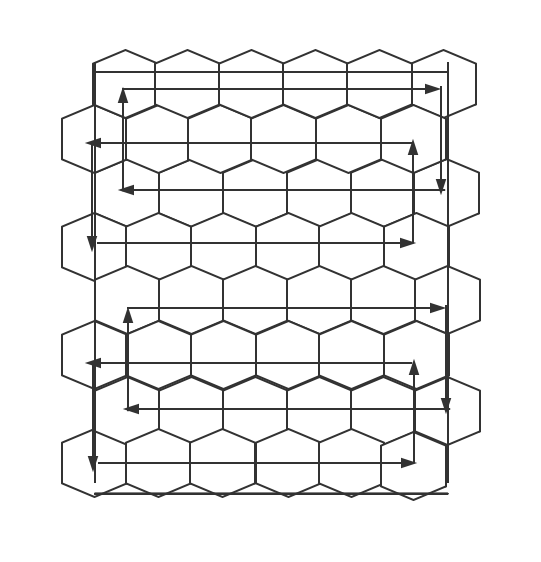
\includegraphics[width=.5\textwidth]{figures/jjj.png}
	\caption{循环运动示意图}\label{jjj}
\end{figure}

\paragraph{结果与分析}
经测算,在高程超过1800m以上的点约占总点数的2.6\%,因此多余面积多占用的无人机架数至多为$0.026*48=1.24$架,误差约为$0.0258$,可以忽略不计。因此把模型简化成全局覆盖有较强的合理性。
	\section{模型的评价}
	\subsection{模型的优点}
	本文通过对飞行路径的全面分析,实现生命游戏算法进行探测路径规划,比群智能算法更容易找到局部最优解,并且时间复杂度仅为$O(n^{2})$;采用优化网格形状为蜂巢密排,使得无人机的利用率进行提高。该模型在实际生活中具有较强的可行性。
	
	\subsection{模型的缺点}
	在对地图进行网格划分的过程中,为简化无人机移动过程中海拔对探测面积的影响与路径规划,造成了部分探测区域的浪费,有一定的改进空间。
	
	\subsection{模型的展望}
	生命游戏算法中无人机是按照指定的路线进行探测,但此路线考虑到高度差后不一定路径最短的优飞行路线,可以通过粒子群优化算法找出一个路径最短的全局最优路线\parencite{hasanipanah2018feasibility},再利用本模型进行探测,从而得到更短的总飞行时间。
	
	\newpage	%换页符
	%%参考文献
	%\begin{thebibliography}{9}%宽度9
	% \setlength{\itemsep}{-2mm}
	
	\printbibliography[title = {参考文献}]	%使用国标参考文献添加方式
	
	% \bibitem{bib:one} 
	% 韩中庚. 数学建模方法及其应用[M]. 高等教育出版社, 2005.
	% \bibitem{bib:two}
	% 韩中庚. 数学建模方法及其应用[M]. 高等教育出版社, 2005.
	% \bibitem{bib:two}
	% 韩中庚. 数学建模方法及其应用[M]. 高等教育出版社, 2005.
	% 
	% \nocite{*}		%排版未引用的参考文献
	% \bibliography{文献数据库}	%不同书库用数据分割
	%
	%\end{thebibliography}
	
	\newpage
	%附录
	\appendix %%附录
\section{代码}
\subsection{数据网格划分并处理--python源代码}
\begin{lstlisting}[language=python]

# author initialize 2019.07.19 00:30:59

import csv

# 数据文件路径
csv_data_file = "height_data.csv"
# 输出文件路径
csv_out_data_file = "output_height_data.csv"
# 列数
col_count = 1165
# 行数
row_count = 874
# cell 宽度 列数
cell_col = 14
# cell 高度 行数
cell_row = 14
# 读取后的数据
height_data = []


if __name__ == "__main__":
print("ready to read")
csv_file = open(csv_data_file)
csv_reader = csv.reader(csv_file)
num_list = [[0] * (col_count) for i in range(row_count)]

i = 0
for row in csv_reader:  # 将csv 转换为 height_data
j = 0
for item in row:
num_list[i][j] = int(item)
j = j + 1
# print(num_list[i])
# time.sleep(1)
i = i + 1

cell_row_num = int(row_count / cell_row)
cell_col_num = int(col_count / cell_col)
print(cell_row_num)
print(cell_col_num)

cell_height_ave_num_list = [[0] * (cell_col_num) for i in range(cell_row_num)]
cell_height_over_2000_num_list = [[0] * (cell_col_num) for i in range(cell_row_num)]

i = 0
for row in num_list:
if int(i / cell_row) >= cell_row_num:
break
j = 0
for item in row:
if int(j / cell_col) >= cell_col_num:
break
cell_height_ave_num_list[int(i / cell_row)][int(j / cell_col)] += item
if item >= 1950:
cell_height_over_2000_num_list[int(i / cell_row)][int(j / cell_col)] += 1
j += 1
i += 1

for i in range(len(cell_height_ave_num_list)):
for j in range(len(cell_height_ave_num_list[0])):
if cell_height_over_2000_num_list[i][j] > 0:
cell_height_ave_num_list[i][j] = -1
else:
cell_height_ave_num_list[i][j] /= (cell_col * cell_row)

# [print(row) for row in cell_height_ave_num_list]
# [print(row) for row in cell_height_over_2000_num_list]

csv_file = open(csv_out_data_file, 'w', newline='')
csv_writer = csv.writer(csv_file, dialect='excel')
for item in cell_height_ave_num_list:
csv_writer.writerow(item)

print("process finished")

\end{lstlisting}
\subsection{等高线图像处理--matlab源代码}
\begin{lstlisting}[language=matlab]

clc, clear, close all
a=xlsread('output.xlsx',1,'A1:ARU874'); %读入高程数据
[m,n]=size(a)
x=0:50:(m-1)*50; y=0:50:(n-1)*50; aa=a';
mesh(x,y,aa) %画三维网格图
title('三维地形图')
figure, contourf(x,y,aa) %画等高线图
colorbar%对等高线添加一个颜色代表的深度
%set(gca,'xticklabel',{''})%x轴刻度不显示
hold on, ax=30000/50, az=a(ax+1,1); 
plot3(30000,0,az,'p','MarkerSize',10,'Color','r') %画出A点位置
text(30500,-200,'A') %标注A点
bx=43000/50; by=30000/50; bz=a(bx+1,by+1);
plot3(43000,30000,bz,'p','MarkerSize',10,'Color','r') %画出B点位置
text(44000,30000,'B'), title('区域的等高线图')

\end{lstlisting}
\subsection{生命游戏算法实现--python源代码}
\begin{lstlisting}[language=python]
#代码被latex混淆了
import numpy as np
import pandas as pd
import math


# 数据文件路径
csv_data_file = "output.csv"
# 列数
col_count = 1165
# 行数
row_count = 874
# cell 宽度 列数
cell_col = 14
# cell 高度 行数
cell_row = 14
# 读取后的数据
height_data = []
#半径
r=353


#a,b的坐标
a_x = 0
a_y = 42
b_x = 41
b_y = 61

#爬山下山损失生命
def cost_life(h1,h2):

cost_d = math.sqrt(h1*h1+h2*h2-2*h1*h2+4*r*r)

return cost_d

#限制a区域最大生命
def limst_A_life(x,y,d):
i = x
j = y
lose = math.sqrt((i-a_x)*(i-a_x)+(j-a_y)*(j-a_y))*2*r
if lose < d:
return True
else:
return False

#限制b区域最大生命
def limst_B_life(x,y,d):
i = x
j = y
lose = math.sqrt((i-b_x)*(i-b_x)+(j-b_y)*(j-b_y))*2*r
if lose < d:
return True
else:
return False

if __name__ == "__main__":
print("ready to read")
data = pd.read_excel('./output.xlsx', header=None)
# print(data.head(5))
A = data[a_x][a_y]
B = data[b_x][b_y]
print(A,B)

#划分数据区域
data_A = data.iloc[:,0:41]
data_B = data.iloc[:,41:]
#print(data_A)

#生命
dd = 600000
e = 10205
dd = dd-e

# 生命
d = dd

#计算飞机上升到最高度
i = a_x
j = a_y
while j > -1:
#往上走一格
j-=1
#坐标
# print("当前坐标("+str(i)+","+str(j)+")")
if(j>-1):
lost = cost_life(data[i][j+i],data[i][j])
d = d - lost
if(limst_A_life(i,j,d)):
pass
else:
print("结束坐标("+str(i)+","+str(j)+")")
break
else:
j+=1
break
print("当前坐标("+str(i)+","+str(j)+")"+",当前生命:"+str(d))

#第一架飞机
flag = 1
while j < 60:
if flag==0:
break

#41为中点的行数
while i < 41:
#往右移动碰壁条件
if data_A[i][j] == -1:
print("碰壁坐标:("+ str(i) + "," + str(j) + ")")
i-=1
break

#往右走一格
i+=1
# 坐标
# print("当前坐标("+str(i)+","+str(j)+")")
if (i < 41):
lost = cost_life(data[i+1][j], data[i][j])
d = d - lost
if (limst_A_life(i, j, d)):
pass
else:
print("结束坐标(" + str(i) + "," + str(j) + ")"+ ",当前生命:" + str(d))
flag = 0
break
else:
i -= 1
break
print("当前坐标(" + str(i) + "," + str(j) + ")" + ",当前生命:" + str(d))

if flag==0:
break

#往下移动一格,损失生命
j += 1
lost = cost_life(data[i][j], data[i][j-1])
d = d - lost

# 从右走到第二条
while i > 0:

# # 往左移动碰壁条件
# if data_A[i][j] == -1:
#     i -= 1
#     break

#往左走一格
i-=1
# 坐标
# print("当前坐标("+str(i)+","+str(j)+")")
if (i > 0):
lost = cost_life(data[i+1][j], data[i][j])
d = d - lost
if (limst_A_life(i, j, d)):
pass
else:
print("结束坐标(" + str(i) + "," + str(j) + ")"+ ",当前生命:" + str(d))
flag = 0
break
else:
i += 1
break
print("当前坐标(" + str(i) + "," + str(j) + ")" + ",当前生命:" + str(d))

if flag==0:
break

# 往下移动一格,损失生命
j += 1
lost = cost_life(data[i][j], data[i][j - 1])
d = d - lost

print("*"*50)

#第二架飞机
#第一架死亡位置(29,28)::往右移动
d = dd
flag = 1#存活
#回到(29,28)距离
lose = math.sqrt((a_x - i) * (a_x - i) + (j - a_y) * (j - a_y)) * 2 * r
d = d -lose
while j < 61:
if flag == 0:
break

# 41为中点的行数
while i < 41:
# 往右移动碰壁条件
if data_A[i][j] == -1:
print("碰壁坐标:(" + str(i) + "," + str(j) + ")")
i -= 1
break

# 往右走一格
i += 1
# 坐标
# print("当前坐标("+str(i)+","+str(j)+")")
if (i < 41):
lost = cost_life(data[i + 1][j], data[i][j])
d = d - lost
if (limst_A_life(i, j, d)):
pass
else:
print("结束坐标(" + str(i) + "," + str(j) + ")" + ",当前生命:" + str(d))
flag = 0
break
else:
i -= 1
break
print("当前坐标(" + str(i) + "," + str(j) + ")" + ",当前生命:" + str(d))

if flag == 0:
break

# 往下移动一格,损失生命
j += 1
lost = cost_life(data[i][j], data[i][j - 1])
d = d - lost

# 从右走到第二条
while i > 0:

# # 往左移动碰壁条件
# if data_A[i][j] == -1:
#     i -= 1
#     break

# 往左走一格
i -= 1
# 坐标
# print("当前坐标("+str(i)+","+str(j)+")")
if (i > 0):
lost = cost_life(data[i + 1][j], data[i][j])
d = d - lost
if (limst_A_life(i, j, d)):
pass
else:
print("结束坐标(" + str(i) + "," + str(j) + ")" + ",当前生命:" + str(d))
flag = 0
break
else:
i += 1
break
print("当前坐标(" + str(i) + "," + str(j) + ")" + ",当前生命:" + str(d))

if flag == 0:
break

# 往下移动一格,损失生命
j += 1
lost = cost_life(data[i][j], data[i][j - 1])
d = d - lost

#第三架飞机
#第二架死亡位置(5,55)::往左移动
d = dd
flag = 1#存活
#回到(5,55)距离
lose = math.sqrt((i - a_x) * (i - a_x) + (j - a_y) * (j - a_y)) * 2 * r
d = d -lose
while j < 61:
if flag == 0:
break

# 从右走到第二条
while i > 0:

# # 往左移动碰壁条件
# if data_A[i][j] == -1:
#     i -= 1
#     break

# 往左走一格
i -= 1
# 坐标
# print("当前坐标("+str(i)+","+str(j)+")")
if (i > 0):
lost = cost_life(data[i + 1][j], data[i][j])
d = d - lost
if (limst_A_life(i, j, d)):
pass
else:
print("结束坐标(" + str(i) + "," + str(j) + ")" + ",当前生命:" + str(d))
flag = 0
break
else:
i += 1
break
print("当前坐标(" + str(i) + "," + str(j) + ")" + ",当前生命:" + str(d))

if flag == 0:
break

# 往下移动一格,损失生命
j += 1
lost = cost_life(data[i][j], data[i][j - 1])
d = d - lost


# 41为中点的行数
while i < 41:
# 往右移动碰壁条件
if data_A[i][j] == -1:
print("碰壁坐标:(" + str(i) + "," + str(j) + ")")
i -= 1
break

# 往右走一格
i += 1
# 坐标
# print("当前坐标("+str(i)+","+str(j)+")")
if (i < 41):
lost = cost_life(data[i + 1][j], data[i][j])
d = d - lost
if (limst_A_life(i, j, d)):
pass
else:
print("结束坐标(" + str(i) + "," + str(j) + ")" + ",当前生命:" + str(d))
flag = 0
break
else:
i -= 1
break
print("当前坐标(" + str(i) + "," + str(j) + ")" + ",当前生命:" + str(d))

if flag == 0:
break
if j==61 :
break

# 往下移动一格,损失生命
j += 1
lost = cost_life(data[i][j], data[i][j - 1])
d = d - lost

print(i,j,d)

# 从右走到第二条
while i > -1:

# # 往左移动碰壁条件
# if data_A[i][j] == -1:
#     i -= 1
#     break

#往左走一格
i-=1
# 坐标
# print("当前坐标("+str(i)+","+str(j)+")")
if (i > -1):
lost = cost_life(data[i+1][j], data[i][j])
d = d - lost
if (limst_A_life(i, j, d)):
pass
else:
print("结束坐标(" + str(i) + "," + str(j) + ")"+ ",当前生命:" + str(d))
flag = 0
break
else:
i += 1
break
print("当前坐标(" + str(i) + "," + str(j) + ")" + ",当前生命:" + str(d))

#回家
while j >= a_y:
#往上走一格
j-=1
#坐标
# print("当前坐标("+str(i)+","+str(j)+")")
if(j>=a_y):
lost = cost_life(data[i][j+i],data[i][j])
d = d - lost
if(limst_A_life(i,j,d)):
pass
else:
print("结束坐标("+str(i)+","+str(j)+")")
break
else:
j+=1
break
print("当前坐标("+str(i)+","+str(j)+")"+",当前生命:"+str(d))
print("小时数:"+str(dd/100000))
\end{lstlisting}
\subsection{计算覆盖率--python源代码}
\begin{lstlisting}[language=python]
import numpy as np
import pandas as pd
import math


# 数据文件路径
csv_data_file = "output.xlsx"

if __name__ == "__main__":
print("ready to read")
data = pd.read_excel(csv_data_file, header=None)
# print(data)

# x=0

S=0
for i in data.columns:
for j in data.index:
# print(data[i][j])
#海拔高度
h = data[i][j]
if(0<h<=2000-math.sqrt(2)*250):
S += 500000
elif(h > 2000-math.sqrt(2)*250):
S += 500*math.sqrt(2)*(4000-2*h)
else:
pass

print("其覆盖面积为:"+str(S))
print("覆盖率为:"+str(S/(43700*58200)))

\end{lstlisting}
\end{document}